
\documentclass[11pt]{exam} % https://www.ctan.org/pkg/exam?lang=en

\usepackage[lmargin=1.in,rmargin=1.in,tmargin=1.in,bmargin=1in]{geometry}
\usepackage{setspace}
\usepackage[pdftex]{graphicx}
\usepackage{titling}
\usepackage[
	pdfauthor={Brian Weinstein},
	pdftitle={Homework 4},
	bookmarks=true,
	colorlinks=true,
	linkcolor=blue,
	urlcolor=blue,
	citecolor=blue,
	pdftex,
	linktocpage=true
	]{hyperref}
\usepackage[textsize=tiny]{todonotes}
\usepackage{float}
\setlength\parindent{0pt}
\usepackage{amsmath}
\usepackage{amssymb}
\usepackage{lipsum}
\usepackage{mathtools}


\qformat{\textbf{Problem \thequestion: \thequestiontitle}\quad \hfill}


\pagestyle{headandfoot}
\runningheadrule
\firstpageheader{}{}{}
\runningheader{\thetitle}{\theauthor}{\thedate}
\firstpagefooter{}{\thepage}{}
\runningfooter{}{\thepage}{}


\usepackage{xcolor}
\usepackage{adjustbox}
\usepackage{verbatim}
\definecolor{shadecolor}{rgb}{.9, .9, .9}

\newenvironment{code}%
   {\par\noindent\adjustbox{margin=1ex,bgcolor=shadecolor,margin=0ex \medskipamount}\bgroup\minipage\linewidth\verbatim}%
   {\endverbatim\endminipage\egroup}

\newenvironment{codeSmall}%
   {\par\noindent\adjustbox{margin=1ex,bgcolor=shadecolor,margin=0ex \medskipamount}\bgroup\minipage\linewidth\verbatim\footnotesize}%
   {\endverbatim\endminipage\egroup}


\newcommand{\argmin}[1]{\underset{#1}{\operatorname{argmin}}\;}




\begin{document}


\title{STAT S4240 002, Homework 4}
\author{Brian Weinstein (bmw2148)}
\date{August 13, 2015}
\maketitle



\begin{questions}



\titledquestion{\href{http://www-bcf.usc.edu/~gareth/ISL/}{James} 6.8.1}

\begin{parts}



\part The model obtained through \textit{best subset selection} has the smallest training RSS for $k \leq p$ predictors. This is because best subset selection tests all possible subsets of size $k$ and chooses the one that minimizes the training RSS.
\smallskip

There is a chance that by using \textit{forward stepwise selection} or \textit{backward stepwise selection} we'd end up with the same optimal subset of $k$ predictors (i.e., the one we obtain via best subset selection), but since the $k$-sized subset is dependent on the covariates included in the prior steps in each of these methods, there's no guarantee that this will be the case.

\part Without either valuating each model on a testing set or estimating test error, none among the three models is guaranteed to have the lowest test RSS. These methods only choose the subset that results in the lowest training RSS, which in no way indicates if the model will also result in a low test RSS.

\part

\begin{subparts}

\subpart True. In a model identified by forward stepwise selection, the subset of predictors in a given step (with $k$ predictors) is the base upon which the next predictor is added in the subsequent step (with $k+1$ predictors).

\subpart True. In a model identified by backward stepwise selection, the subset of predictors in a given step (with $k$ predictors) is itself a subset of the predictors used in the previous step (with $k+1$ predictors).

\subpart False. The forward stepwise and backward stepwise models using $k$ predictors are not guaranteed to use the same subset of predictors. As such, once an additional variable is added to the forward stepwise model (or equivalently, once a variable is removed from the backward stepwise model), there's no guarantee that the variables in the $k$-variable backward stepwise model are a subset of the $k+1$-variable forward stepwise model.

\subpart False, with similar reasoning to Part (iii). The $k$ predictors in a forward stepwise model are the predictors that, at each incremental step, kept the error as low as possible. Similarly, the $k+1$ predictors in a backward stepwise model are the predictors at each incremental step that kept the error as low as possible. Since each subset of predictors depends on those used in the previous step, there's no guarantee (although it may happen to be the case) that a set of predictors obtained via forward selection is a subset of those obtained via backward selection.

\subpart False. The set of $k$ predictors chosen in best subset selection are those that keep the error in the $k$-variable model as low as possible. Independently, the set of $k+1$ predictors chosen in best subset are those that keep the error in the $k+1$-variable model as low as possible. There's no guarantee that $k$ of the variables included in the $(k+1)$-variable model are those that minimize the error in the $k$-variable model.


\end{subparts}
 

\end{parts}



\titledquestion{\href{http://www-bcf.usc.edu/~gareth/ISL/}{James} 6.8.3}

Estimating the regression coefficients in a linear regression model via

$$\argmin{\hat{\beta}}\left\{ \sum_{i=1}^{n} \left(    y_i - \beta_0 - \sum_{j=1}^p \beta_j x_{ij} \right) \right\} \quad \text{subject to} \quad \sum_{j=1}^p \left|{\beta_j}\right| \leq s$$

for a given value of $s$.

%is equivalent to estimating the coefficients via
%$$\argmin{\hat{\beta}}\left\{ \sum_{i=1}^{n} \left(    y_i - \beta_0 - \sum_{j=1}^p \beta_j x_{ij} \right)  + \lambda \sum_{j=1}^p \left|{\beta_j}\right|\right\}.$$

As we increase $s$ from 0:

\begin{parts}

\part The training RSS will (\textbf{iv.}) steadily decrease. As we make the constraint on $\sum_{j=1}^p \left|{\beta_j}\right|$ less strict, the limitation on the size of $\hat{\beta}$ disappears and we eventually get the standard ``least residuals'' solution. At $s=0$ we start with only the intercept $\beta_0$ non-zero. As we increase $s$ we allow for additional non-zero coefficients, eventually including all coefficients in the model. With all coefficients included, we minimize the training error (while potentially overfitting).


\part The testing RSS will (\textbf{ii.}) decrease initially, and then eventually start increasing in a U shape. At $s=0$ we start with a highly-biased model with only the intercept $\beta_0$ non-zero. As we increase $s$ we allow for \textit{some} of the $\beta_{j\neq0}$ to take non-zero values (since the constraint is the same as that used in the lasso), which reduces the bias and increases the variance, for an overall drop in RSS. Once we increase $s$ enough, \textit{all} of the $\beta_{j\neq0}$ will take non-zero values and we're left with a model with very low bias, but very high variance, increasing the RSS.

\part The variance will (\textbf{iii.}) steadily increase. The reasoning here is similar to that used in Part (ii): At $s=0$ we start with a very inflexible model, and as we increase $s$ to allow more non-zero coefficients, the model flexibility, and thus our variance, increases.

\part The (squared) bias will (\textbf{iv.}) steadily decrease. The reasoning here is similar to that used in Part (ii): At $s=0$ we start with a highly-biased, very inflexible model with only one coefficient, $\beta_0$. As we increase $s$ to allow more non-zero coefficients, the model flexibility, and thus our squared bias, decreases.

\part The irreducible error will (\textbf{v.}) remain constant. The irreducible error is a function of the data we're given, not the model we choose, so our choice of $s$ has no effect on the size of the irreducible error.

\end{parts}



\titledquestion{\href{http://www-bcf.usc.edu/~gareth/ISL/}{James} 6.8.5}

\textit{It is well-known that ridge regression tends to give similar coefficient values to correlated variables, whereas the lasso may give quite different coefficient values to correlated variables. We will now explore this property in a very simple setting.
Suppose that $n = 2$, $p = 2$, $x_{11} = x_{12}$, $x_{21} = x_{22}$. Furthermore, suppose that $y_1+y_2 =0$ and $x_{11}+x_{21} =0$ and $x_{12}+x_{22} =0$, so that the estimate for the intercept in a least squares, ridge regression, or lasso model is zero: $\hat{\beta}_0 = 0$.}

\begin{parts}

\part \textit{Write out the ridge regression optimization problem in this setting.}

$$  \sum_{i=1}^{n} \left( y_i - \beta_0 - \sum_{j=1}^{p} \beta_j x_{ij}  \right)^2       + \lambda  \sum_{j=1}^{p} \beta_j^2   $$

Since $n=2$, $p=2$, and $\beta_0=0$,
$$  \sum_{i=1}^{2} \left( y_i - 0 - \sum_{j=1}^{2} \beta_j x_{ij}  \right)^2       + \lambda  \sum_{j=1}^{2} \beta_j^2   .$$


Expanding the summations,
$$   \left(  y_1 - \beta_1 x_{11} - \beta_2 x_{12}  \right)^2  + \left(  y_2 - \beta_1 x_{21} - \beta_2 x_{22}  \right)^2  + \lambda \beta_1^2  +  \lambda \beta_2^2  .$$


And since $\left( x_{11}=x_{12}=-x_{21}=-x_{22} \coloneqq x\right)$ and $\left( y_1 = -y_2 \coloneqq y \right)$,

$$   
\left(  y - \left( \beta_1 + \beta_2 \right) x \right)^2 + \left( - y + \left( \beta_1 + \beta_2 \right) x \right)^2   + \lambda \left( \beta_1^2 + \beta_2^2 \right)   .$$

Then expanding the polynomial terms and simplifying,
$$ 2y^2 - 4xy \left( \beta_1 + \beta_2 \right) + 2 x^2 \left( \beta_1 + \beta_2 \right)^2 + \lambda \left( \beta_1^2 + \beta_2^2 \right) \coloneqq \mathcal{L}.$$







\part \textit{Argue that in this setting, the ridge coefficient estimates satisfy $\hat{\beta}_1 = \hat{\beta}_2$.}

\smallskip

Taking the derivative of $\mathcal{L}$ with respect to $\hat{\beta}_1$,
$$\frac{\partial \mathcal{L}}{\partial \hat{\beta}_1} = -4xy+4x^2\hat{\beta}_1 + 4x^2\hat{\beta}_2 + 2\lambda\hat{\beta}_1 = 0 ,$$

and taking the derivative of $\mathcal{L}$ with respect to $\hat{\beta}_2$,
$$\frac{\partial \mathcal{L}}{\partial \hat{\beta}_2} = -4xy+4x^2\hat{\beta}_1 + 4x^2\hat{\beta}_2 + 2\lambda\hat{\beta}_2 = 0.$$


Equating $\frac{\partial \mathcal{L}}{\partial \hat{\beta}_1} = \frac{\partial \mathcal{L}}{\partial \hat{\beta}_2}$ (since both $=0$) yields:
$$-4xy+4x^2\hat{\beta}_1 + 4x^2\hat{\beta}_2 + 2\lambda\hat{\beta}_1 = -4xy+4x^2\hat{\beta}_1 + 4x^2\hat{\beta}_2 + 2\lambda\hat{\beta}_2$$  
$$ \Rightarrow \hat{\beta}_1 = \hat{\beta}_2$$





\part \textit{Write out the lasso optimization problem in this setting.}


$$  \sum_{i=1}^{n} \left( y_i - \beta_0 - \sum_{j=1}^{p} \beta_j x_{ij}  \right)^2       + \lambda  \sum_{j=1}^{p} \left|\beta_j\right|   $$

Since $n=2$, $p=2$, and $\beta_0=0$,
$$  \sum_{i=1}^{2} \left( y_i - 0 - \sum_{j=1}^{2} \beta_j x_{ij}  \right)^2       + \lambda  \sum_{j=1}^{2} \left|\beta_j\right|   .$$


Expanding the summations,
$$   \left(  y_1 - \beta_1 x_{11} - \beta_2 x_{12}  \right)^2  + \left(  y_2 - \beta_1 x_{21} - \beta_2 x_{22}  \right)^2  + \lambda \left|\beta_1\right|  +  \lambda \left|\beta_2\right|  .$$


And since $\left( x_{11}=x_{12}=-x_{21}=-x_{22} \coloneqq x\right)$ and $\left( y_1 = -y_2 \coloneqq y \right)$,

$$   
\left(  y - \left( \beta_1 + \beta_2 \right) x \right)^2 + \left( - y + \left( \beta_1 + \beta_2 \right) x \right)^2   + \lambda \left( \left|\beta_1\right| + \left|\beta_2\right| \right)   .$$

Then expanding the polynomial terms and simplifying,
$$ 2y^2 - 4xy \left( \beta_1 + \beta_2 \right) + 2 x^2 \left( \beta_1 + \beta_2 \right)^2 + \lambda \left( \left|\beta_1\right| + \left|\beta_2\right| \right) \coloneqq \mathcal{L}.$$

























\part \textit{Argue that in this setting, the lasso coefficients $\hat{\beta}_1$ and $ \hat{\beta}_2$ are not unique---in other words, there are many possible solutions to the optimization problem in (c). Describe these solutions.}

\smallskip

Taking the derivative of $\mathcal{L}$ with respect to $\hat{\beta}_1$,
$$\frac{\partial \mathcal{L}}{\partial \hat{\beta}_1} = -4xy+4x^2\hat{\beta}_1 + 4x^2\hat{\beta}_2 + \lambda \frac{\partial}{\partial \hat{\beta}_1} \left| \hat{\beta}_1 \right|= 0 ,$$

and taking the derivative of $\mathcal{L}$ with respect to $\hat{\beta}_2$,
$$\frac{\partial \mathcal{L}}{\partial \hat{\beta}_2} = -4xy+4x^2\hat{\beta}_1 + 4x^2\hat{\beta}_2 + \lambda \frac{\partial}{\partial \hat{\beta}_2} \left| \hat{\beta}_2 \right|= 0 .$$


Equating $\frac{\partial \mathcal{L}}{\partial \hat{\beta}_1} = \frac{\partial \mathcal{L}}{\partial \hat{\beta}_2}$ (since both $=0$) yields:
$$-4xy+4x^2\hat{\beta}_1 + 4x^2\hat{\beta}_2 + \lambda \frac{\partial}{\partial \hat{\beta}_2} \left| \hat{\beta}_2 \right| = -4xy+4x^2\hat{\beta}_1 + 4x^2\hat{\beta}_2 + \lambda \frac{\partial}{\partial \hat{\beta}_2} \left| \hat{\beta}_2 \right|$$ 

 
$$ \Rightarrow \frac{\partial}{\partial \hat{\beta}_1} \left| \hat{\beta}_1 \right| = \frac{\partial}{\partial \hat{\beta}_2} \left| \hat{\beta}_2 \right|$$

The presence of the absolute values indicate that there are \textit{at least} two possible values for each $\hat{\beta}_1$ and $\hat{\beta}_2$.






\end{parts}



\titledquestion{\href{http://www-bcf.usc.edu/~gareth/ISL/}{James} 8.4.5}

10 bootstrapped samples produces estimates of $P\left( \textrm{Class is Red}|X  \right)$ that yield 0.1, 0.15, 0.2, 0.2, 0.55, 0.6, 0.6, 0.65, 0.7, and 0.75.

Based on the majority vote approach, we'd classify this $X$ as Red, since 6 of the 10 estimates have probabilities greater than 0.5.

Based on the average probability approach, we'd classify this $X$ as Green, since the average probability from our 10 samples is 0.45 ($<0.5$).




\titledquestion{Federalist Papers Classification with Trees}

\begin{parts}

\part Gini Impurity Coefficient Splits

\begin{subparts}

\subpart Model Assessment

\begin{code}
  accuracy falseNegRate falsePosRate
1 0.962963            0   0.09090909
\end{code}

\begin{itemize}
\item Accuracy: \% of test papers that are classified correctly
\item False Negative Rate: \% of Hamilton papers incorrectly classified as Madison
\item False Positive Rate: \% of Madison papers incorrectly classified as Hamilton
\end{itemize}


\subpart Tree Plot

\begin{figure}[H]
	\centering
	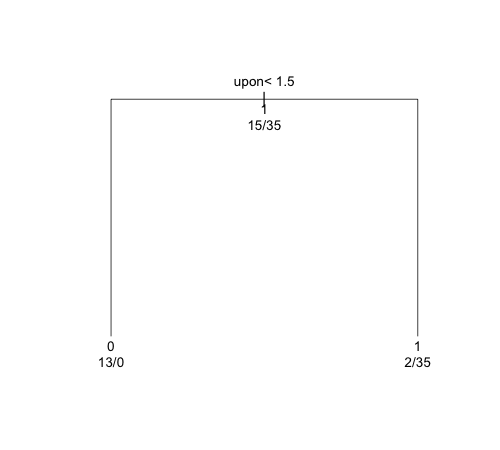
\includegraphics[width=350px]{5a.png}
	%\caption{}
	%\label{fig:figName}
\end{figure}

\end{subparts}



\part Information Gain Splits

\begin{subparts}

\subpart Model Assessment

\begin{code}
  accuracy falseNegRate falsePosRate
1 0.962963            0   0.09090909
\end{code}

\subpart Tree Plot

\begin{figure}[H]
	\centering
	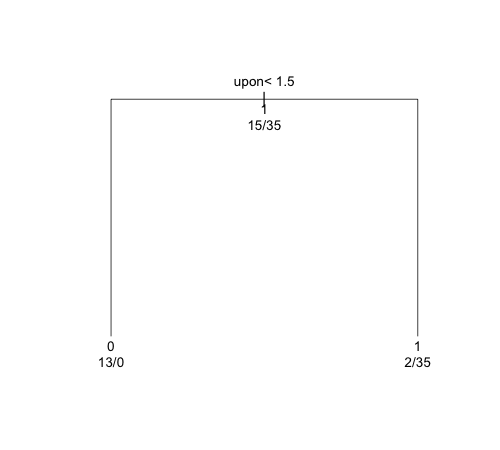
\includegraphics[width=350px]{5b.png}
	%\caption{}
	%\label{fig:figName}
\end{figure}


\subpart The trees generated from Gini Impurity Coefficient splits and Information Gain splits ended up being identical here.


\end{subparts}




\end{parts}







\titledquestion{Federalist Papers Classification with Regularized Logistic Regression}

\begin{parts}

\part We should always center and scale our data whenever we us use a regularization method. Without scaling our data, the variables with larger values would have smaller coefficients (to indicate some level of importance), which would decrease the penalty for these predictors. Similarly, variables with smaller values would have much larger coefficients (to indicate the same level of importance), which would increase the penalty for these predictors.
\smallskip

In our dataset, since each of the word counts are on different scales (i.e., some words are much more common than others), performing unregularized logistic regression wouldn't penalize each of the variables in a comparable way.



\part Ridge Regression

\begin{subparts}

\subpart Model Assessment

\begin{code}
   accuracy falseNegRate falsePosRate
1 0.5925926            0            1
\end{code}

\subpart Important Words

The 10 words with the largest coefficients (in absolute value) are shown below.
\begin{code}
       word        coef    absCoef
1  februari -0.01667849 0.01667849
2      upon  0.01572523 0.01572523
3    whilst -0.01428038 0.01428038
4    within -0.01367440 0.01367440
5     sever -0.01344406 0.01344406
6      1783 -0.01302052 0.01302052
7      form -0.01193143 0.01193143
8    member -0.01168190 0.01168190
9         5 -0.01153821 0.01153821
10 although -0.01127392 0.01127392
\end{code}

\end{subparts}






\part Lasso

\begin{subparts}

\subpart Model Assessment

\begin{code}
   accuracy falseNegRate falsePosRate
1 0.8888889            0    0.2727273
\end{code}

\subpart Important Words

The 10 words with the largest coefficients (in absolute value) are shown below.
\begin{code}
       word       coef   absCoef
1    whilst -1.3557246 1.3557246
2  februari -1.1650795 1.1650795
3      upon  1.1493109 1.1493109
4      form -0.5714197 0.5714197
5  although -0.4741114 0.4741114
6    within -0.4227536 0.4227536
7     sever -0.3698089 0.3698089
8    lesser -0.3483888 0.3483888
9      anim -0.1694737 0.1694737
10 indirect -0.1641048 0.1641048
\end{code}

Both ridge and lasso include ``februari'', ``upon'', ``whilst'', ``within'', ``sever'', ``form'', and "although'' in the their 10 most important words.
\smallskip

``1783'', ``member'', and ``5'' are included in the top 10 ridge words, but not in the top 10 lasso; and ``lesser'', ``anim'', and ``indirect'' are included in lasso, but not in ridge.
\smallskip

In general the ridge weights are smaller (in absolute value) than those from lasso.

\end{subparts}


\end{parts}






\titledquestion{Federalist Papers Classification with Feature Selection}

\begin{parts}

\part \todo{Problem 7}

\end{parts}



\titledquestion{\href{http://www-bcf.usc.edu/~gareth/ISL/}{James} 8.4.10}

Using boosting to predict \texttt{Salary} in the \texttt{Hitters} data set.

\begin{parts}

\part Removing the observations with no salary information, and log-transforming the salaries.
\begin{code}
# remove observations with no salary info
Hitters <- Hitters[!is.na(Hitters$Salary), ]

# log transform the salaries
Hitters$Salary <- log(Hitters$Salary) #$
\end{code}


\part Creating training and testing sets.

\begin{code}
Hitters.train <- Hitters[1:200, ]
Hitters.test <- Hitters[-(1:200), ]
\end{code}



\part Boosting on the training set with 1,000 trees for a range of values of the shrinkage parameter $\lambda \in \left\{  0.0001, 0.0051, 0.0101, 0.0151, \ldots, 0.2951      \right\}$. Training MSE vs $\lambda$ shown below.

\begin{figure}[H]
	\centering
	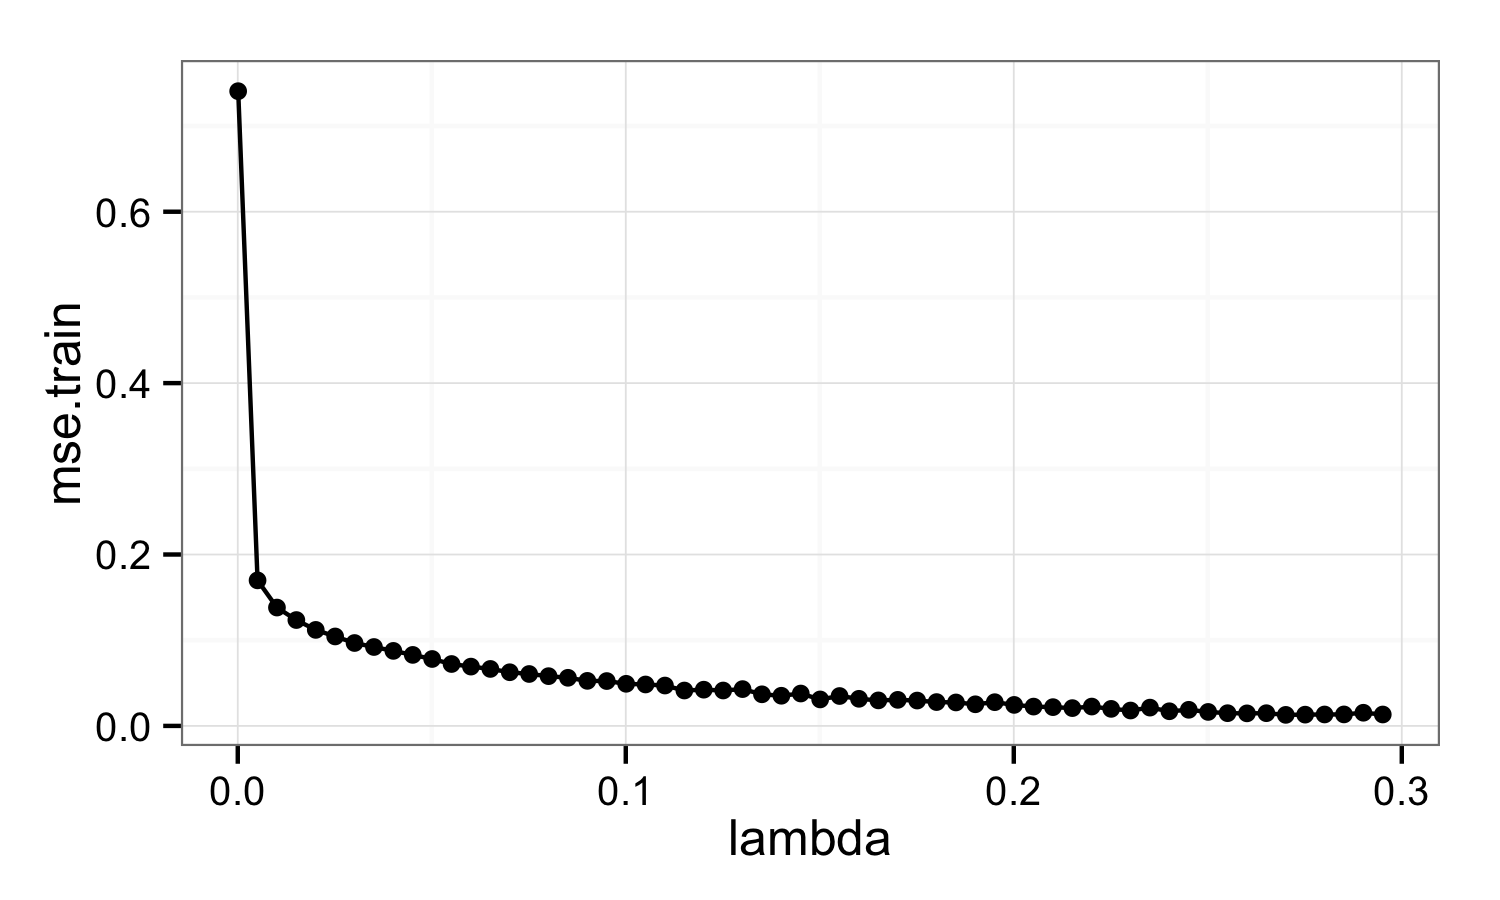
\includegraphics[width=5in]{8c_trainMSE.png}
	%\caption{}
	%\label{fig:figName}
\end{figure}


\part Boosting on the training set with 1,000 trees for a range of values of the shrinkage parameter $\lambda \in \left\{  0.0001, 0.0051, 0.0101, 0.0151, \ldots, 0.2951      \right\}$. Test MSE vs $\lambda$ shown below.

\begin{figure}[H]
	\centering
	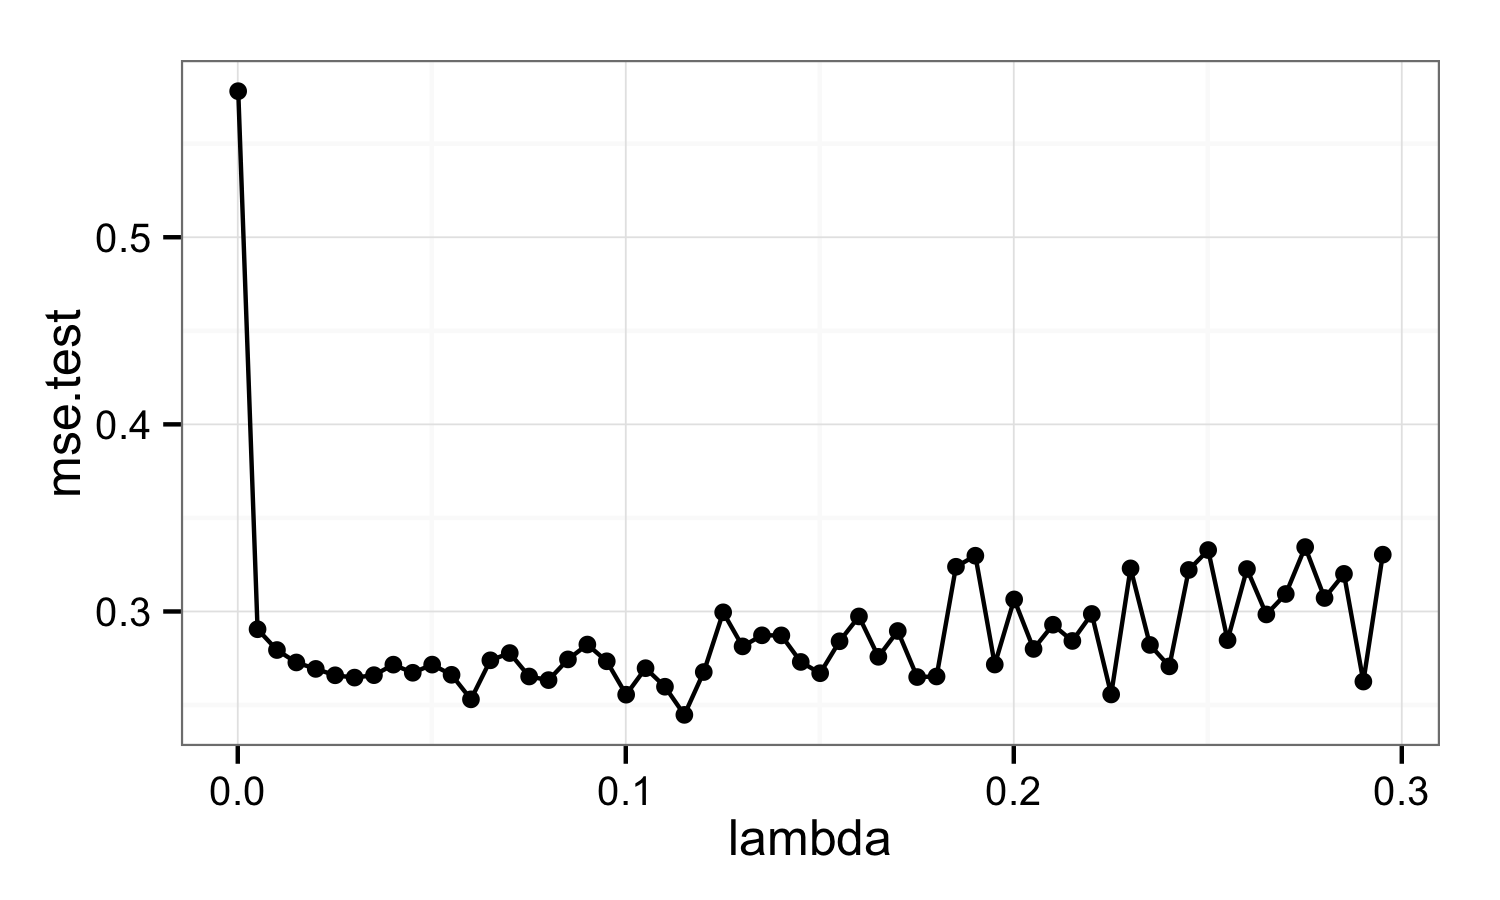
\includegraphics[width=5in]{8d_testMSE.png}
	%\caption{}
	%\label{fig:figName}
\end{figure}


\part Boosting generates a test MSE of 0.2447458 (at $\lambda=0.1151$). I compared the boosting MSE to the errors obtained from OLS regression (from Chapter 3) and the lasso (from Chapter 6).
\smallskip

OLS regression generated a test MSE of $0.4918959$:
\indent \begin{code}
model.ols <- lm(formula = Salary ~ ., data=Hitters.train)
pred.test.ols <- predict(model.ols, newdata=Hitters.test)
mse.test.ols <- mean((Hitters.test$Salary - pred.test.ols)^2) #$
\end{code}
\smallskip

And the lasso generates a test MSE of $0.4696547$:
\begin{codeSmall}
model.lasso <- cv.glmnet(x=model.matrix(Salary ~ ., Hitters.train)[, -1],
                         y=Hitters.train$Salary,
                         alpha=1, family="gaussian",
                         type.measure="mse")
pred.test.lasso <-  predict(model.lasso, newx=model.matrix(Salary ~ ., Hitters.test)[, -1],
                            s="lambda.min", type="response")
mse.test.lasso <- mean((Hitters.test$Salary - (as.data.frame(pred.test.lasso)$"1"))^2) #$
\end{codeSmall}
\smallskip

The boosting approach generates a significantly lower test MSE than OLS regression and the lasso.




\part In the boosted model, \texttt{CAtBat} is by far the most important predictor. \texttt{PutOuts} is the second most important, but has less than half the relative influence of \texttt{CAtBat}. The relative influence statistics of all variables in the model are shown below.

\begin{code}
                var     rel.inf
CAtBat       CAtBat 23.57153591
PutOuts     PutOuts  9.01152161
CHits         CHits  8.57868893
Walks         Walks  7.15658743
Years         Years  6.15196246
CRuns         CRuns  5.54809666
RBI             RBI  5.51043189
CRBI           CRBI  5.20052999
CHmRun       CHmRun  4.86688069
Assists     Assists  4.27511089
AtBat         AtBat  4.08888482
Hits           Hits  3.86999152
HmRun         HmRun  3.45383623
CWalks       CWalks  2.62813762
Errors       Errors  2.56909410
Runs           Runs  2.23166814
NewLeague NewLeague  0.66480707
Division   Division  0.52425937
League       League  0.09797467
\end{code}



\part Bagging generates a test MSE of $0.2309305$, which is slightly better than the test MSE obtained through the boosting and much better than the MSEs obtained through OLS regression and the lasso.

\begin{codeSmall}
# train the model
model.bag <- randomForest(formula = Salary ~ .,
                          data=Hitters.train,
                          mtry=(ncol(Hitters.train) - 1), # consider *all* variables in
                                                          # each split (bagging)
                          ntree=1000,
                          importance=TRUE)

# use model to predict values for the testing data
pred.test.bag <- predict(model.bag,
                         newdata=Hitters.test[, -which(colnames(Hitters.test)=="Salary")])

# calculate the testing MSE
mse.test.bag <- mean((Hitters.test$Salary - pred.test.bag)^2) #$
\end{codeSmall}









\end{parts}



\titledquestion{\href{http://www-bcf.usc.edu/~gareth/ISL/}{James} 10.7.1}

\textit{This problem involves the K-means clustering algorithm.}

\begin{parts}

\part \textit{Prove (10.12)}

$$\frac{1}{\left| C_k \right|}  \sum_{i,i^\prime \in C_k } \sum_{j=1}^p       \left(  x_{ij} - x_{i^\prime j}   \right)^2    =  2 \sum_{i \in C_k } \sum_{j=1}^p   \left(  x_{ij} - \bar{x}_{kj} \right)^2 . $$

\begin{figure}[H]
	\centering
	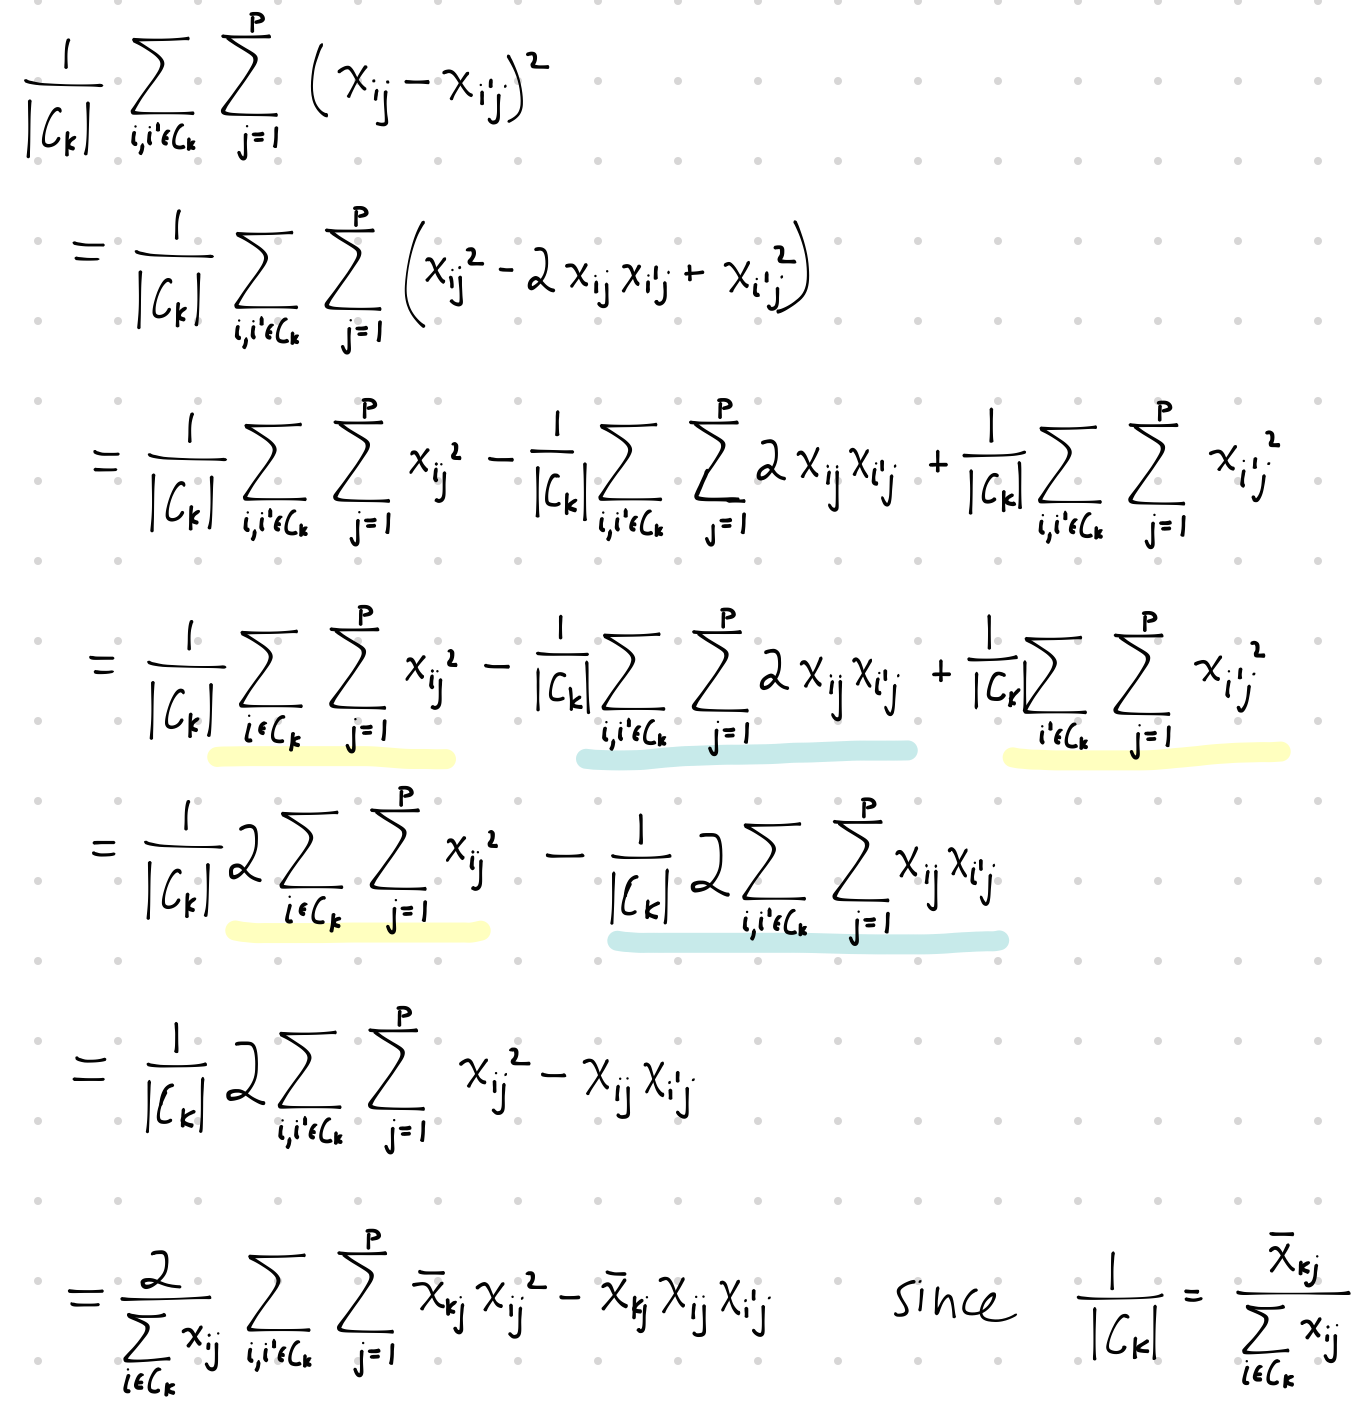
\includegraphics[width=6in]{9a.png}
	%\caption{}
	%\label{fig:figName}
\end{figure}

\todo{fix and type up 9a}

\part \textit{On the basis of this identity, argue that the K-means clustering algorithm (Algorithm 10.1) decreases the objective (10.11) at each iteration.}

The right side of Equation (10.12) is proportional to the sum of the Euclidean distances between each point in a cluster and the cluster's centroid.
\smallskip

In step 2b of Algorithm 10.1, each observation is assigned to the centroid that is closest to it, which either decreases the right side of (10.12) or leaves it unchanged.
\smallskip

By the identity in (10.12), step 2b must also decrease $\frac{1}{\left| C_k \right|}  \sum_{i,i^\prime \in C_k } \sum_{j=1}^p       \left(  x_{ij} - x_{i^\prime j}   \right)^2$, which is the within-cluster variation for the $k$th cluster.

The objective in (10.11) minimizes the sum of the within-cluster variations for all $K$ clusters, and thus Algorithm (10.1) decreases the objective in (10.11).

\end{parts}





\end{questions}




%\begin{figure}[H]
%	\centering
%	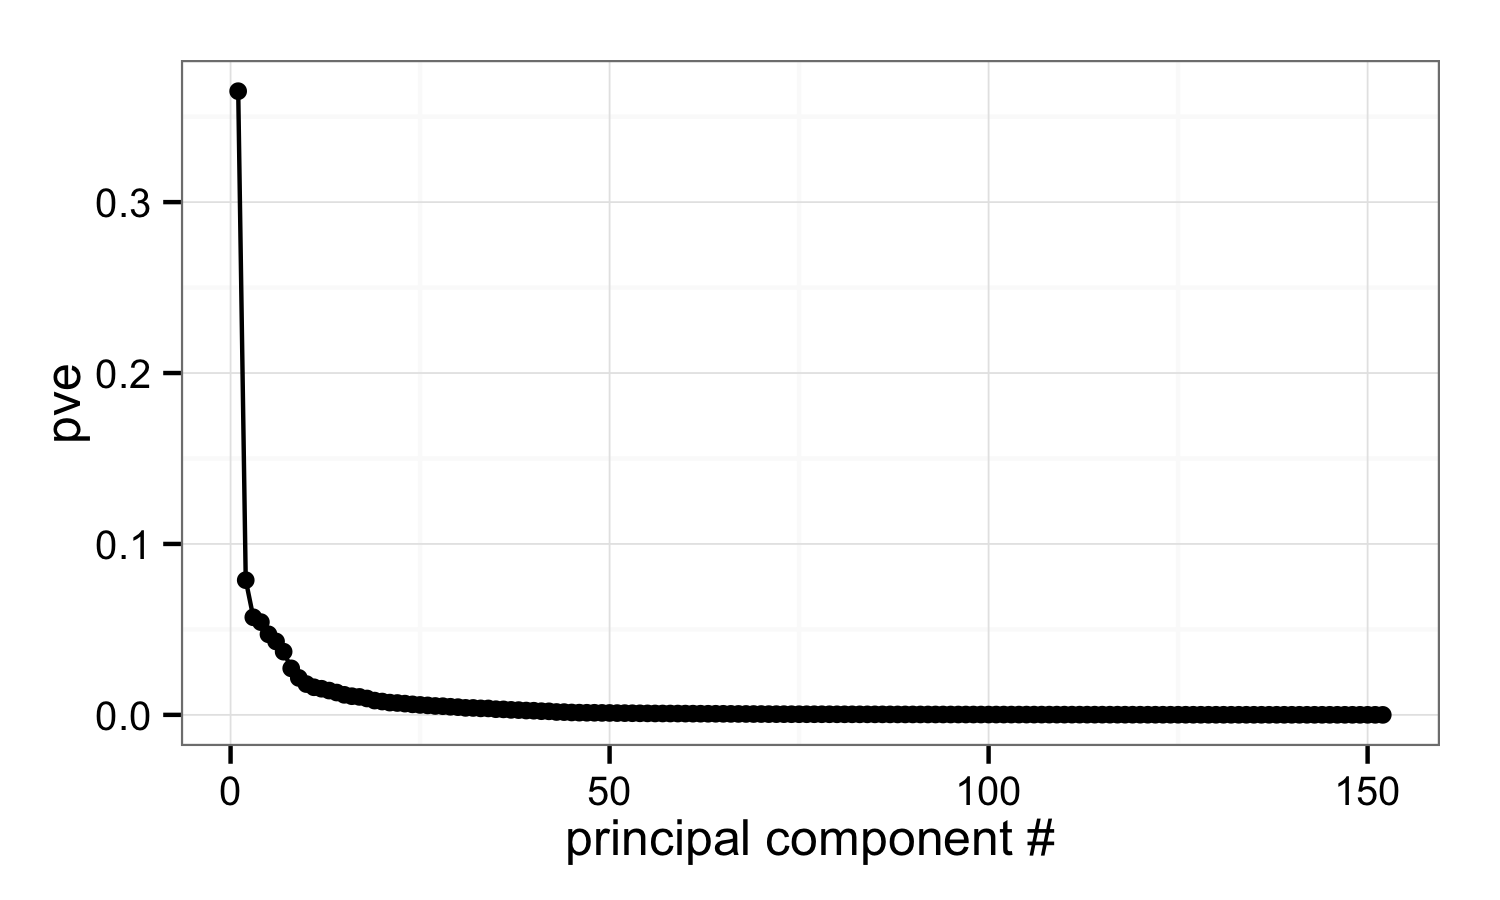
\includegraphics[width=5in]{2c.png}
%	%\caption{}
%	%\label{fig:figName}
%\end{figure}




%\listoftodos

\end{document}